\documentclass[12pt,italian]{report}
\usepackage{tesi}

%
%			INFORMAZIONI SULLA TESI
%			DA COMPILARE!
%

% CORSO DI LAUREA:
\def\myCDL{Corso di Laurea magistrale in\\Informatica}
% TITOLO TESI:
\def\myTitle{Il titolo\\della tesi}

% AUTORE:
\def\myName{Lorenzo D'Alessandro}
\def\myMat{Matr. Nr. 939416}

% RELATORE E CORRELATORE:
\def\myRefereeA{Relatore 1}
\def\myRefereeB{Correlatore 1}

% ANNO ACCADEMICO
\def\myYY{2020-2021}

% Il seguente comando introduce un elenco delle figure dopo l'indice (facoltativo)
%\figurespagetrue

% Il seguente comando introduce un elenco delle tabelle dopo l'indice (facoltativo)
%\tablespagetrue

%
%			PREAMBOLO
%			Inserire qui eventuali package da includere o definizioni di comandi personalizzati
%

% Package di formato
\usepackage[a4paper]{geometry}		% Formato del foglio
\usepackage[italian]{babel}			% Supporto per l'italiano
\usepackage[utf8]{inputenc}			% Supporto per UTF-8
%\usepackage[a-1b]{pdfx}			% File conforme allo standard PDF-A (obbligatorio per la consegna)

% Package per la grafica
\usepackage{graphicx}				% Funzioni avanzate per le immagini
\usepackage{hologo}					% Bibtex logo with \hologo{BibTeX}
%\usepackage{epsfig}				% Permette immagini in EPS
%\usepackage{xcolor}				% Gestione avanzata dei colori

% Package tipografici
\usepackage{amssymb,amsmath,amsthm} % Simboli matematici
\usepackage{listings}				% Scrittura di codice

% Package ipertesto
\usepackage{url}					% Visualizza e rendere interattii gli URL
\usepackage{hyperref}				% Rende interattivi i collegamenti interni


\begin{document}

% Creazione automatica del frontespizio
\frontespizio
\beforepreface

% 
%			PAGINA DI DEDICA E/O CITAZIONE
%			facoltativa, questa è l'unica cosa che dovete formattare a mano, un po' come vi pare
%

{\raggedleft \large \sl Dedica \\}
         
% 
%			PREFAZIONE (facoltativa)
%

%\prefacesection{Prefazione}
%Le prefazioni non sono molto comuni, tuttavia a volte capita che qualcuno voglia dire qualcosa che esuli dal lavoro in s\'e (come un meta-commento sull'elaborato), o voglia fornire informazioni riguardanti l'eventuale progetto entro cui la tesi si colloca (in questo caso \`e probabile che sia il relatore a scrivere questa parte).

%
%			RINGRAZIAMENTI (facoltativi)
%

\prefacesection{Ringraziamenti}
Questa sezione, facoltativa, contiene i ringraziamenti.

%
%			Creazione automatica dell'indice
%

\afterpreface

% 
%			CAPITOLO 1: Introduzione o Abstract
% 

\chapter{Introduzione}
\label{cap:introduzione}

Introduzione...

\section{I contenuti}
\label{sec:contenuti}

Spiegazione problema...


\section{Organizzazione della tesi}
\label{sec:organizzazione}

Organizzazione tesi...

% 
%			CAPITOLO 2: Stato dell'arte
% 

\chapter{Stato dell'arte}
\label{chap:stato_arte}



% 
%			CAPITOLO 3: Lavoro svolto
% 

\chapter{Classificatore}
\label{chap:classificatore}

\section{Limitazioni recsys collaborative filtering}
La principale limitazione dei recommender system dei collaborative filtering è definire il numero di users e items prima di iniziare l'aggiornamento/training del modello. Nel caso degli algoritmi di matrix factorization la matrice di input è composta da un numero di righe pari al numero di users, e un numero di colonne pari al numero di items. Nel caso dei modelli basati su reti neurali descritti nel \autoref{chap:stato_arte} è necessario dare in input ai modelli le lunghezze dei vettori di users e items che corrispondono rispettvamente al numero di users e items.

In entrambi se si vuole aggiungere un nuovo user/item è necessario ricompilare il modello ed eseguire nuovamente da zero la fase di training. Questo non è un problema in un ambiente desktop in cui è possibile aggiornare giornalmente lato server le preferenze di tutti gli utenti con una cadenza regolare (es. una volta al giorno).

Eseguire di nuovo il traning da zero ogni volta che nuovi users/items vengono scoperti è un problema se si vuole fare il traning direttamente su dispositivo mobile. In questo caso c'è un problema sia di dispendio energetico, sia di tempo effettivo per il traing.

\section{Struttura classificatore}
Il modello proposto in questa tesi è una rete feed-forward fully-connected. Una rete feed-forward non contiene cicli nel suo grafo \cite{Goodfellow-et-al-2016}, mentre fully connected indica che ogni neurone in un layer è connesso a tutti i neuroni del layer successivo. Il numero di layer nascosti e il numero di neuroni in ogni layer è stato deciso nella fase di tuning descritta nel \autoref{chap:risultati}.
Il numero di neuroni nel layer di output è sempre 1 come è prassi nei problemi di classificazione binaria. La funzione di attivazione scelta per i layer nascosti è ReLU (rectified linear unit), che è più plausibile biologicamente rispetto ad altre funzioni come sigmoide hyperbolic tangent, non viene saturata e aiuta a prevenire l'overfitting del modello \cite{rectifier-neural-networks}. La funzione di attivazione scelta per il layer di output è la sigmoide che limita l'output a valori compresi tra 0 e 1. La funzione di loss della rete è binary cross entropy.

\begin{figure}
  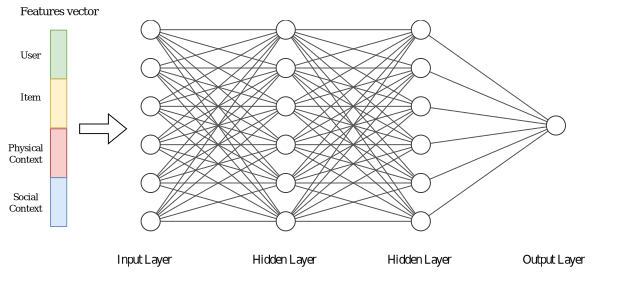
\includegraphics[width=\linewidth]{immagini/ffnet_schema.png}
  \caption{Schema rete feed-forward}
  \label{fig:ffnet_schema}
\end{figure}

% 
%			CAPITOLO 4: Datasets
% 

\chapter{Datasets}
\label{chap:datasets}


% 
%			CAPITOLO 5: Risultati
% 

\chapter{Risultati}
\label{chap:risultati}


% 
%			CAPITOLO 6: Conclusioni e sviluppi futuri
% 

\chapter{Conclusioni}
\label{cap6}

\section{Conclusioni}

Conclusioni...

\section{Sviluppi futuri}

Sviluppi futuri...



%
%			BIBLIOGRAFIA
%

\bibliographystyle{unsrt}
\bibliography{bibliografia}
\nocite{*}
\addcontentsline{toc}{chapter}{Bibliografia}


\end{document}


 
